\documentclass{article}

\usepackage{amsmath}
\usepackage{amssymb}
\usepackage{graphicx}

\setlength\parindent{0pt}

\newcommand{\norm}[1]{\left\lVert#1\right\rVert}
\newcommand*\mean[1]{\bar{#1}}

\renewcommand{\thefootnote}{\fnsymbol{footnote}}

\DeclareMathOperator*{\argmax}{arg\,max}
\DeclareMathOperator*{\mmax}{max}
\DeclareMathOperator*{\argmin}{arg\,min}

\begin{document}

\title{Definitions and notations}
\author{Zhehao Wang}

\maketitle{}

\section{Calculus and linear algebra}

\subsection{Limit}

Let $f(x)$ be a function defined on an interval that contains $x = a$, except possibly at $x = a$, then we say that
$$
\lim\limits_{x \to a}{f(x) = L}
$$
if for every $\epsilon > 0$ there is some number $\delta > 0$ such that
$$
|f(x) - L| < \epsilon ~ \text{whenever} ~ 0 < |x - a| < \delta
$$

\subsection{Gradient}
Given $f(\vec{x})$ where $\vec{x} = (x_1, \dots, x_n)$ on $\mathbb{R}^n$
$$
\bigtriangledown f(a_1, \dots, a_n) = (\frac{\partial f}{\partial x_1}(a_1, \dots, a_n), \dots, \frac{\partial f}{\partial x_n}(a_1, \dots, a_n))
$$

\textbf{Intuition}: gradient is a vector (the rate of change of your function, when you move in a certain direction), which in a two-dimensional space, tangents the curve at a given point.

\subsection{Directional derivative}

\textbf{Homework notation}
$$
f'(x; u) = \lim\limits_{h \to 0}{\frac{f(x + hu) - f(x)}{h}}
$$

\textbf{Wikipedias notation}

$$
\bigtriangledown_v f(\vec{x}) = \lim\limits_{h \to 0}{\frac{f(\vec{x} + h\vec{v}) - f(\vec{x})}{h}}
$$

\textbf{Intuition}: the rate-of-change of a function $f(\vec{x})$ on direction $\vec{v}$.
Remember that this is a scalar (since we are given the direction).

$$
f'(x; u) = \bigtriangledown f(x)^{T} u
$$

Meaning gradient on a certain direction vector $u$ is $f(x)$'s directional derivative on $u$.

\subsection{Vector norm}
A norm is a function that assigns a stricly positive length or size to each vector in a vector space (except the zero vector which is assigned a length of 0).

\textbf{Absolute value norm} is a norm on the one-dimensional vector spaces formed by real or complex numbers.
$$
\norm{x} = |x|
$$

\textbf{Euclidean norm} on a Euclidean space $\mathbb{R}^n$ is such
$$
\norm{\vec{x}}_2 = \sqrt{x_1^2 + \dots + x_n^2}
$$

\textbf{Manhattan or taxicab norm}
$$
\norm{\vec{x}}_1 = \sum_{i = 1}^{n}{|x_i|}
$$

\textbf{$p$-norm}
$$
\norm{\vec{x}}_p = (\sum_{i = 1}^{n}{|x_i|^p})^{\frac{1}{p}}
$$
Note that when $p = 1$, we get Manhattan norm, and when $p = 2$, we get Euclidean norm.

When $p = \infty$
$$
\norm{\vec{x}}_{\infty} = {\mmax_{i}{|x_i|}}
$$

\subsection{argmax}

Points of the domain of some function at which the function values are maximized.

Given an arbitrary set $X$, a totally ordered set $Y$ and a function $f: X \to Y$, the $\argmax$ over some subset $S$ of $X$ is defined by
$$
\argmax_{x \in S \subseteq X}{f(x)} = \{x ~ | ~ x \in S \land \forall y \in S : f(y) \leq f(x)\}
$$

\subsection{Dot product, inner product}

Maps two equal-size vectors to a real value.

$$
\cdot : \mathbb{R}^d \times \mathbb{R}^d \to \mathbb{R}
$$

Defined geometrically, given two vectors $a$ and $b$,

$$
a \cdot b = \norm{a} \norm{b} cos(\theta)
$$

where $\theta$ is the angle between $a$ and $b$.

Defined algebraically,

$$
a \cdot b = a^{T}b
$$

\subsection{Cauchy-Schwarz inequality}

Given two vectors $u$ and $v$

$$
|\langle u , v \rangle|^2 \leq |\langle u , u \rangle| \cdot |\langle v , v \rangle|
$$

Where $|\langle u , u \rangle|$ is the inner product.
The equality holds only when $u$ and $v$ are linearly independent (parallel).

\subsection{Jacobian matrix}

\textbf{Jacobian matrix} is the matrix of all first-order partial derivatives of a vector-valued function.

Suppose $\vec{f} : \mathbb{R}^n \to \mathbb{R}^m$, the Jacobian matrix $\vec{J}$ of $\vec{f}$ is defined as follows

$$
\vec{J} = \begin{bmatrix} ~ \frac{\partial \vec{f}}{\partial x_1} ~ \dots ~ \frac{\partial \vec{f}}{\partial x_n} ~ \end{bmatrix}
$$

or component-wise $\vec{J}_{ij} = \frac{\partial \vec{f_i}}{\partial x_j}$, meaning

$$
\vec{J} = 
 \begin{bmatrix}
  \frac{\partial \vec{f_1}}{\partial x_1} ~ \dots ~ \frac{\partial \vec{f_1}}{\partial x_n} \\
  \dots \\
  \frac{\partial \vec{f_m}}{\partial x_1} ~ \dots ~ \frac{\partial \vec{f_m}}{\partial x_n}
 \end{bmatrix}
$$

\subsection{Order of a matrix}



\subsection{Inversibility of a matrix}



\subsection{Eigenvalue, eigenvector}

An \textbf{eigenvalue} of a \textbf{linear transformation} \footnote{Think square transformation matrix} is a non-zero vector that changes by only a scalar factor when that linear transformation is applied to it.

Meaning the set of $\vec{v}$ that satisfies

$$
T(\vec{v}) = \lambda \vec{v}
$$

Where $T$ is the linear transformation, $\lambda$ is a scalar and called \textbf{eigenvalue}.

We can compute the eigenvalues $\lambda$ of a square matrix $A$ of size $n$ by solving this \textbf{determinant}

$$
|A - \lambda I| = 0
$$

Where $I$ is the \textbf{identity matrix (unit matrix)} of size $n$.

For each eigenvalue $\lambda$, we can then solve its (corresponding set of) eigenvectors $\vec{v}$ using

$$
(A - \lambda I) \cdot \vec{v} = 0
$$

\textbf{Intuition}: applying a linear transformation on an eigenvector of that linear transformation yields a vector that is parallel to this eigenvector (multiplier: eigenvalue).

\subsection{Positive-definite}

A \textbf{symmetric} $n \times n$ real matrix is positive definite if the scalar $z^{T} M z$ is strictly positive for every non-zero column vector $z \in \mathbb{R}^n$.

The identity matrix $I$ is positive definite.

For any real invertible matrix $A$, the product $A^{T} A$ is a positive definite matrix.

\section{Probability}

\subsection{Random variable}

A random variable $X : \Omega \to \mathit{E}$ is a measurable function from a set of possible outcomes $\Omega$ to a measurable space $\mathit{E}$.
Often times $\mathit{E} = \mathbb{R}$

The probability that $X$ takes on a value in a measurable set $S \subseteq \mathit{E}$ is written as
$$
Pr(X \in S) = P({\omega \in \Omega | X(\omega) \in S})
$$

\textbf{Intuition}: mapping outcomes of a random process to numbers, like this definition of $X$
$$
X =
\begin{cases}
0, & \text{if heads} \\
1, & \text{if tails}
\end{cases}
$$
Instead of a traditional algebraic variable that can be solved for one value, a random variable can have different values (each with a probability) under different conditions.

\subsection{Law of large numbers}
\label{law-of-large-numbers}

$X_i, X_2, \dots$ is an infinite sequence of independent and identically distributed (iid) random variables with expected value $E(X_1) = E(X_2) = \dots = \mu$, and
$$
\mean{X}_n = \frac{1}{n}(X_1 + \dots + X_n) ~ \footnote{What does the sum of random variables mean? Seems that each $X_i$ here means 'sampled' values following the distribution defined by the random variable, like, the outcome of an experiment}
$$


\textbf{The weak law} states that for any positive number $\epsilon$
$$
\lim\limits_{n \to \infty}{Pr(|\mean{X}_n - \mu| > \epsilon)} = 0
$$

\textbf{The strong law} states that
$$
Pr(\lim\limits_{n \to \infty}{\mean{X}_n = \mu}) = 1
$$

\textbf{Intuition}: law of large numbers is a theorem that describes the average of the results obtained from a large number of trials should be close to the expected value, and will tend to become closer as more trials are performed.


\section{Statistical learning}

Let $\mathbf{X}$ denote the input space, $\mathbf{Y}$ denote the output space, and $\mathbf{A}$ denote the action space.

A \textbf{decision function / prediction function} $f: \mathbf{X} \to \mathbf{A}$ maps an input to an action.

A \textbf{loss function} $\mathit{l}: \mathbf{A} \times \mathbf{Y} \to \mathbb{R}$ evaluates an action in the context of an output, and maps the error to a real.
In traditional problems we can usually assume action has no effect on the output (like stock market prediction).

\subsection{Risk, Bayesian function, empirical risk}

Assume there is a data generating distribution $P_{\mathbf{X} \times \mathbf{Y}}$.

\textbf{Risk} of a decision function can then be defined as
$$
R(f) = \mathbb{E}\mathit{l}(f(x), y)
$$
Where an input/output pair $(x, y)$ is generated independently and identically distributed from $P_{\mathbf{X} \times \mathbf{Y}}$.

A \textbf{Bayesian decision function / target function} $f^* : \mathbf{X} \to \mathbf{A}$ is a function that achieves the minimal risk among all possible functions.
$$
f^* = \argmin_{f}{R(f)}
$$

Risk cannot be calculated as we are not given $P_{\mathbf{X} \times \mathbf{Y}}$.

Let $\mathbf{D}_n = \{(x_1, y_1), \dots, (x_n, y_n)\}$ be drawn iid from $P_{\mathbf{X} \times \mathbf{Y}}$.

The \textbf{empirical risk} of $f : \mathbf{X} \to \mathbf{A}$ with respect to $\mathbf{D}_n$ is

$$
\hat{R}_n(f) = \frac{1}{n} \sum_{i = 1}^{n}{\mathit{l}(f(x_i), y_i)}
$$

By strong law of large numbers (\ref{law-of-large-numbers}), when $n$ is big enough, empirical risk can be used to approximate risk.

\subsection{Empirical risk minimization, constrained empirical risk minimization}

A function $\hat{f}$ is an \textbf{empirical risk minimizer} if
$$
\hat{f} = \argmin_{f}{\hat{R}_n(f)}
$$
The prediction function that produces the smallest empiricall risk over set $\mathbf{D}_n$.
This naturally leads to overfit.

So we minimize empirical risk, but only within a hypothesis space $\mathbf{F}$, being a set of prediction functions.

\textbf{Constrained empirical risk minimizer} can then be defined as
$$
\hat{f}_n = \argmin_{f \in \mathbf{F}}{\frac{1}{n} \sum_{i = 1}^{n}{\mathit{l}(f(x_i), y_i)}}
$$

If we plug Risk in instead, a \textbf{constrained risk minimizer} becomes
$$
f^*_{\mathbf{F}} = \argmin_{f \in \mathbf{F}}{\mathbb{E}\mathit{l}(f(x), y)}
$$

\textbf{Approximation error} is the risk difference between the constrained risk minimizer (in $\mathbf{F}$) and the target

$$
R(f_{\mathbf{F}}) - R(f^*)
$$

\textbf{Estimation error} is the risk difference between the constrained empirical risk minimizer and the constrained risk minimizer (both in $\mathbf{F}$)

$$
R(\hat{f}_n) - R(f_{\mathbf{F}})
$$

\textbf{Optimization error} is the risk difference between a function $\tilde{f}_n$ (which we find in practice) and the constrained empirical risk minimizer
\footnote{Optimization can be negative, however, this $\hat{R}(\tilde{f}_n) - \hat{R}(\hat{f}_n)$ can't.
In this hypothesis space, this function can fit the overall world better than the constrained empirical risk minimizer, but it can't on the training set, on which the constrained ERM performs best in this space}

$$
R(\tilde{f}_n) - R(\hat{f}_n)
$$

\textbf{Excess risk} is the risk between a function and the target
$$
\text{Excess Risk}(\hat{f}_n) = \text{Estimation Error} + \text{Approximation Error} = R(\hat{f}_n) - R(f^*)
$$
\begin{align*}
\text{Excess Risk}(\tilde{f}_n) &= \text{Optimization Error} + \text{Estimation Error} + \text{Approximation Error} \\
                                &= R(\tilde{f}_n) - R(f^*)
\end{align*}

\subsection{Complexity measure, $\mathit{l}_1$, $\mathit{l}_2$ regularization, ridge regression, lasso regression, coordinate gradient descent}

\textbf{Regularization} is a mechanism to reduce overfitting.
By narrowing down the hypothesis space to only those functions who satisfies being within a complexity measure (or penalize the empirical risk minimizer with another term representing complexity).

\textbf{Complexity measure} $\Omega : \mathbf{F} \to [0, \infty)$ for linear decision functions $f(x) = w^{T} x$ can be defined using the $p$-norm (to the $p$) of $w$.

\begin{itemize}
  \item $\mathit{l}_0$ complexity is then the number of non-zero coefficients
  \item $\mathit{l}_1$ \textbf{lasso} complexity is $\sum_{i = 1}^{d}{|w_i|}$
  \item $\mathit{l}_2$ \textbf{ridge} complexity is $w^{T} w = \sum_{i = 1}^{d}{w_{i}^{2}}$
\end{itemize}

To factor complexity measure in constrained empirical risk minimization, we can use \textbf{Ivanov} or \textbf{Tikhonov} regularization. where

$$
\argmin_{f \in \mathbf{F}}{\frac{1}{n} \sum_{i = 1}^{n}{\mathit{l}(f(x_i), y_i)}} ~ \text{s.t.} ~ \Omega(f) \leq r
$$

is Ivanov regularization, and

$$
\argmin_{f \in \mathbf{F}}{\frac{1}{n} \sum_{i = 1}^{n}{\mathit{l}(f(x_i), y_i)} + \lambda \Omega(f)}
$$

is Tikhonov regularization.
The two can be shown to be equivalent for many performance measure of $f$, and $\Omega$, using Lagrangian duality theory.

Plugging in the lasso / ridge definition of $\Omega$ to either form, we get lasso / ridge regression.

For example, ridge regression in Tikhonov form looks like

$$
\hat{w} = \argmin_{w \in \mathbb{R}^{d}}{\frac{1}{n} \sum_{i = 1}^{n}{(w^{T} x_i - y_i)^2} + \lambda \norm{w}_2^2}
$$

Lasso regression typically lead to feature sparsity (more coefficient equal to $0$).
This can be shown intuitively by comparing the two on the intersection of contour plot (of empirical risk minimizer) and the area constrained by lasso (diamond on a $f(x) = ax + b$ prediction function) / ridge (circle on the same prediction function) regression, as show in Figure \ref{lasso-vs-ridge-sparsity}\footnote{https://niallmartin.wordpress.com/2016/05/12/shrinkage-methods-ridge-and-lasso-regression/}.

\begin{figure}[h]
\centering
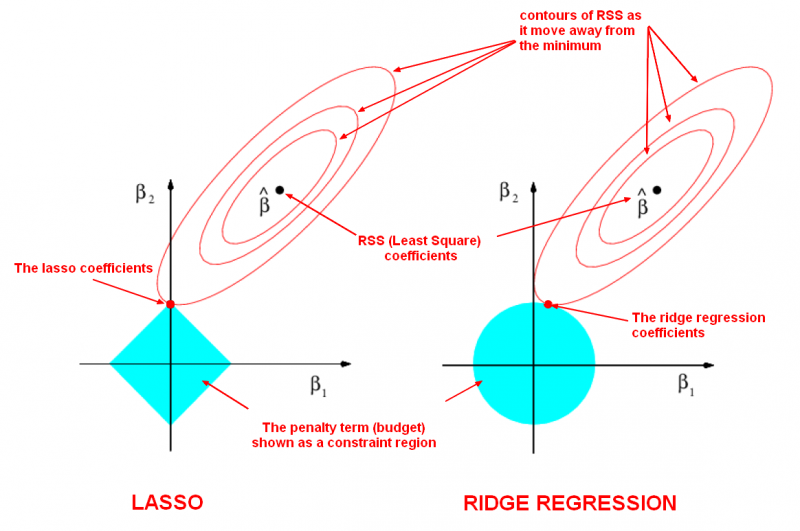
\includegraphics[scale=0.3]{res/lasso_vs_ridge_regression.png}
\caption{Why lasso regression tends to lead to feature sparsity}
\label{lasso-vs-ridge-sparsity}
\end{figure}

Lasso regression ($\mathit{l}_1$-norm) is not differentiable, thus we cannot apply gradient descent as-is.
We split each coefficient into positive and negative parts: rewrite the vector $w = w^{+} - w^{-}$ ($|w| = w^{+} + w^{-}$), and we have this equivalent problem\footnote{whose equivalence can be proved. And this can be plugged in to a quadratic solver to give us $w^{+}$ and $w^{-}$}:

$$
\argmin_{w^{+}, w^{-}}{\frac{1}{n} \sum_{i = 1}^{n}{((w^{+} - w^{-})^{T} x_i - y_i)^2} + \lambda (w^{+} + w^{-})}
$$
subject to $w_i^{+} \geq 0 ~ \forall i$, $w_i^{-} \leq 0 ~ \forall i$

Now we have a constraint and two vectors, to find the minimum, we can use \textbf{projected SGD}\footnote{Normal gradient descent but project / reset each coordinate to the constrained space after each step} or \textbf{coordinate descent}.

Coordinate gradient descent on a vector $w$ works by adjusting only a single $w_i$ in each step, as opposed to possibly alter the entire $w$ in one step as in regular gradient descent.
We iteratively adjust each coordinate several times, where we can pick a random one to adjust, or do cyclic adjustment.

Coordinate gradient descent has a \textbf{closed form solution} for lasso (in the form below\footnote{This form is not differentiable, but it can be shown that for coordinate gradient descent to work there is a weaker condition, which lasso satisfies. \textit{This would indicate that the split into positive and negative shown above is not required, for solving using coordinate gradient descent?}}), where we can use a formula to solve each $w_i$, instead of having to loop over them.

$$
\hat{w}_j = \argmin_{w_j \in \mathbb{R}}{\frac{1}{n} \sum_{i = 1}^{n}{(w^{T} x_i - y_i)^2} + \lambda \norm{w}_1}
$$

\subsection{Elastic nets}

Consider what happens in lasso and ridge regressions when features are linear:
lasso would assign all the weight to the feature with larger scale, and ridge would assign the weights proportional to the features' scales.

It's similar when features are highly correlated (near-linear relationship between features):
think Figure \ref{lasso-vs-ridge-sparsity} instead of parallel lines, we get elongated ellipses, whose intersection with the hypothesis space would reflect the scales of correlated features.

\textbf{Elastic net} combines lasso and ridge penalties.

$$
\hat{w} = \argmin_{w \in \mathbb{R}^{d}}{\frac{1}{n} \sum_{i = 1}^{n}{(w^{T} x_i - y_i)^2} + \lambda_1 \norm{w}_1 + \lambda_2 \norm{w}_2^2}
$$

Geometrically, we end with a hypothesis space like a diamond with edges bulging out (between a circle and a diamond).

\subsection{Regression loss functions}

A \textbf{distance-based loss function} is a loss function ($\mathit{l}(\hat{y}, y) \in \mathbb{R}$) that only depends on the \textbf{residual} $r = \hat{y} - y$.
Most regression losses are distance-based.

Distance-based losses are translation-invariant: $\mathit{l}(\hat{y} + a, y + a) = \mathit{l}(\hat{y}, y)$.

Square loss ($\mathit{l}(r) = r^2$) penalizes outlier points more heavily than absolute (Laplacian) loss ($\mathit{l} = |r|$) does, and is considered less robust.

Downside with absolute loss is that it's not differentiable.

We are able to construct \textbf{Huber loss function} that is robust and differentiable: quadratic for $|r| \leq \delta$ and linear for $|r| > \delta$.

\subsection{Classification loss functions}

If we have action space $\mathbf{A}$ and outcome space $\mathbf{Y}$ both being $\{-1, 1\}$.

\textbf{0-1 loss} for $f: \mathbf{X} \to \{-1, 1\}$:

$$
\mathit{l}(f(x), y) = 1 ~ (f(x) \neq y)
$$

Where $1 ~ (f(x) \neq y)$ denotes score 1 whenever $(f(x) \neq y)$.
\\
\\
If we allow \textbf{real-valued prediction function} $f : \mathbf{X} \to \mathbb{R}$, meaning action space $\mathbf{A} = \mathbb{R}$ where the value represents confidence of our prediction.

We can define \textbf{margin} $m$ as $m = y \hat{y}$.
We want to maximize the margin.
Most classification losses are \textbf{margin-based}.

Empirical risk for 0-1 loss is

$$
\hat{R}_n(f) = \frac{1}{n} \sum_{i = 1}^{n}{1}~(y_i f(x_i) \leq 0)
$$

$\hat{R}_n(f)$ is non-convex, not differentiable, discontinuous, and its optimization is NP-hard.
\\
\\
\textbf{SVM/Hinge loss} is defined as

$$
\mathit{l}_{Hinge} = max\{ 1 - m, 0 \} = (1 - m)_+
$$

It is a convex, upper bound on 0-1 loss, and not differentiable at $m = 1$.
And we have \textbf{margin error} when $m < 1$.

Using hinge loss function, we define \textbf{soft margin linear support vector machine} (a constrained empirical risk minimizer) as

$$
\argmin_{w \in \mathbb{R}^{d}}{\frac{1}{n} \sum_{i = 1}^{n}{(1 - y_i f_w (x_i))_+} + \lambda \norm{w}_2^2}
$$

With $l2$ regularization, and hypothesis space is linear $\{f(x) = w^{T} x | w \in \mathbb{R}^d\}$.
\\
\\
\textbf{Logistic/log loss} is defined as 

$$
\mathit{l}_{Logistic} = \text{log}(1 + e^{-m})
$$

It always wants more margin, and is differentiable.
\\
\\
0-1 loss, hinge and Logistic loss functions are illustrated in Figure \ref{logistic-hinge-01-loss} \footnote{http://fa.bianp.net/blog/2013/loss-functions-for-ordinal-regression/}.

\begin{figure}[h]
\centering
\includegraphics[scale=0.3]{res/logistic-hinge-01-loss.png}
\caption{0-1 loss, hinge loss and Logistic loss functions}
\label{logistic-hinge-01-loss}
\end{figure}


\section{Exercises}

\subsection{Deriving gradient affine form}

1. Given $f(w) = c^{t} w$ , $\bigtriangledown f(w)$?

$$
f'(x; u) = \lim\limits_{h \to 0}{\frac{f(w + hu) - f(w)}{h}} = \lim\limits_{h \to 0}{\frac{c^{T} h u}{h}} = c^{T} u
$$

This shows

$$
\bigtriangledown f(x) = c
$$

2. Given $f(w) = w^{T} A w$ , $\bigtriangledown f(w)$?

\begin{align*}
f'(w; u) &= \lim\limits_{h \to 0}{\frac{f(w + hu) - f(w)}{h}} \\
         &= \lim\limits_{h \to 0}{\frac{(w + hu)^{T} A (w + hu) - w^{T} A w}{h}} \\
         &= \lim\limits_{h \to 0}{ \frac{w^{T} A w + h w^{T} u + h u^{T} A w + h^2 u^{T} A u - w^{T} A w}{h} } \\
         &= u^{T} A w + w^{T} A u \\
         &= w^{T} A^{T} u + w^{T} A u
\end{align*}

This shows
$$
\bigtriangledown f(x) = (w^{T} A^{T} + w^{T} A)^{T} = (A + A^{T}) w
$$

3. Given $f(w) = \norm{Aw - y}_2^2$ , $\bigtriangledown f(w)$?

$$
f(w) = \norm{Aw - y}_2^2 = (Aw - y)^{T} (Aw - y)
$$

\begin{align*}
f'(w; u) &= \lim\limits_{h \to 0}{\frac{(A (w + hu) - y)^{T} (A (w + hu) - y) - (Aw - y)^{T} (Aw - y)}{h}} \\
         &= \lim\limits_{h \to 0}{ (A (w + hu) - y)^{T} A u + (A u)^{T} (A (w + hu) - y)} \\
         &= (A w - y)^{T} A u + (A u)^{T} (A w - y) \\
         &= 2 (A w - y)^{T} A u
\end{align*}

This shows

$$
\bigtriangledown f(x) = 2 ((A w - y)^{T} A)^{T} = 2 A^{T} (A w - y) = 2 A^{T} A w - 2 A^{T} y
$$

4. Given $f(w) = \norm{Aw - y}_2^2 + \lambda \norm{w}_2^2$ , express $f(w) = \norm{Bw - z}_2^2$?

The gradient of the two need to be the same, using previous result, we need to solve

$$
\begin{cases}
A^{T} A + \lambda &= B^{T} B \\
          A^{T} y &= B^{T} z
\end{cases}
$$

Note the equivalence between extending a matrix and addition, let

$$
B = \begin{pmatrix} A \\ \sqrt{\lambda} I_{n \times n} \end{pmatrix} ~ \text{and} ~ z = \begin{pmatrix} y \\ 0_{n \times 1} \end{pmatrix}
$$

written in block-matrix form.

\subsection{Recap: linear regression with square loss}


\end{document}
